% Created by tikzDevice version 0.12.6 on 2026-10-29 12:50:27
% !TEX encoding = UTF-8 Unicode
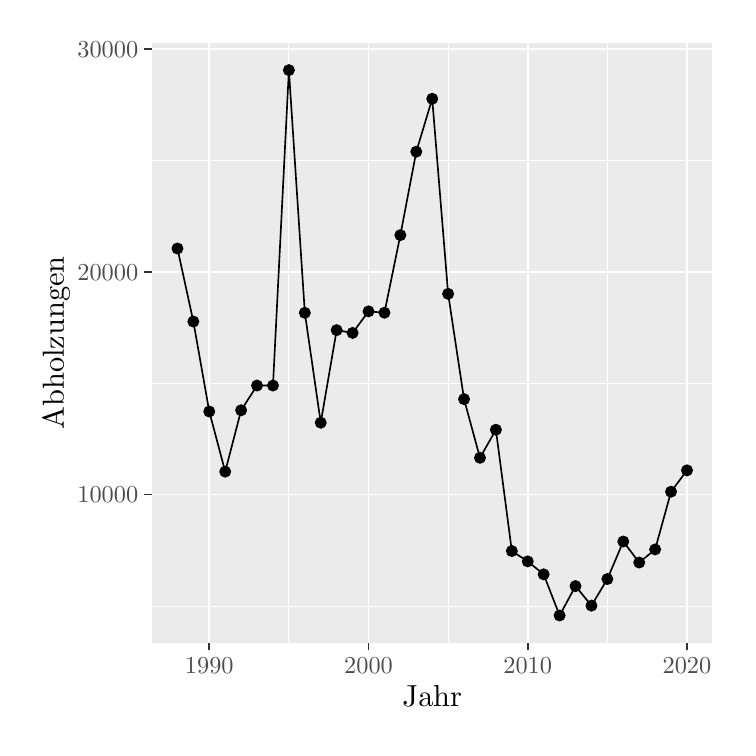
\begin{tikzpicture}[x=1pt,y=1pt]
\definecolor{fillColor}{RGB}{255,255,255}
\path[use as bounding box,fill=fillColor,fill opacity=0.00] (0,0) rectangle (252.94,252.94);
\begin{scope}
\path[clip] (  0.00,  0.00) rectangle (252.94,252.94);
\definecolor{drawColor}{RGB}{255,255,255}
\definecolor{fillColor}{RGB}{255,255,255}

\path[draw=drawColor,line width= 0.6pt,line join=round,line cap=round,fill=fillColor] (  0.00,  0.00) rectangle (252.94,252.94);
\end{scope}
\begin{scope}
\path[clip] ( 44.91, 30.69) rectangle (247.44,247.45);
\definecolor{fillColor}{gray}{0.92}

\path[fill=fillColor] ( 44.91, 30.69) rectangle (247.44,247.45);
\definecolor{drawColor}{RGB}{255,255,255}

\path[draw=drawColor,line width= 0.3pt,line join=round] ( 44.91, 43.99) --
	(247.44, 43.99);

\path[draw=drawColor,line width= 0.3pt,line join=round] ( 44.91,124.46) --
	(247.44,124.46);

\path[draw=drawColor,line width= 0.3pt,line join=round] ( 44.91,204.93) --
	(247.44,204.93);

\path[draw=drawColor,line width= 0.3pt,line join=round] ( 94.39, 30.69) --
	( 94.39,247.45);

\path[draw=drawColor,line width= 0.3pt,line join=round] (151.93, 30.69) --
	(151.93,247.45);

\path[draw=drawColor,line width= 0.3pt,line join=round] (209.47, 30.69) --
	(209.47,247.45);

\path[draw=drawColor,line width= 0.6pt,line join=round] ( 44.91, 84.23) --
	(247.44, 84.23);

\path[draw=drawColor,line width= 0.6pt,line join=round] ( 44.91,164.69) --
	(247.44,164.69);

\path[draw=drawColor,line width= 0.6pt,line join=round] ( 44.91,245.16) --
	(247.44,245.16);

\path[draw=drawColor,line width= 0.6pt,line join=round] ( 65.62, 30.69) --
	( 65.62,247.45);

\path[draw=drawColor,line width= 0.6pt,line join=round] (123.16, 30.69) --
	(123.16,247.45);

\path[draw=drawColor,line width= 0.6pt,line join=round] (180.70, 30.69) --
	(180.70,247.45);

\path[draw=drawColor,line width= 0.6pt,line join=round] (238.24, 30.69) --
	(238.24,247.45);
\definecolor{drawColor}{RGB}{0,0,0}
\definecolor{fillColor}{RGB}{0,0,0}

\path[draw=drawColor,line width= 0.4pt,line join=round,line cap=round,fill=fillColor] ( 54.12,173.14) circle (  1.96);

\path[draw=drawColor,line width= 0.4pt,line join=round,line cap=round,fill=fillColor] ( 59.87,146.75) circle (  1.96);

\path[draw=drawColor,line width= 0.4pt,line join=round,line cap=round,fill=fillColor] ( 65.62,114.24) circle (  1.96);

\path[draw=drawColor,line width= 0.4pt,line join=round,line cap=round,fill=fillColor] ( 71.38, 92.51) circle (  1.96);

\path[draw=drawColor,line width= 0.4pt,line join=round,line cap=round,fill=fillColor] ( 77.13,114.69) circle (  1.96);

\path[draw=drawColor,line width= 0.4pt,line join=round,line cap=round,fill=fillColor] ( 82.88,123.62) circle (  1.96);

\path[draw=drawColor,line width= 0.4pt,line join=round,line cap=round,fill=fillColor] ( 88.64,123.62) circle (  1.96);

\path[draw=drawColor,line width= 0.4pt,line join=round,line cap=round,fill=fillColor] ( 94.39,237.59) circle (  1.96);

\path[draw=drawColor,line width= 0.4pt,line join=round,line cap=round,fill=fillColor] (100.15,149.90) circle (  1.96);

\path[draw=drawColor,line width= 0.4pt,line join=round,line cap=round,fill=fillColor] (105.90,110.19) circle (  1.96);

\path[draw=drawColor,line width= 0.4pt,line join=round,line cap=round,fill=fillColor] (111.65,143.64) circle (  1.96);

\path[draw=drawColor,line width= 0.4pt,line join=round,line cap=round,fill=fillColor] (117.41,142.64) circle (  1.96);

\path[draw=drawColor,line width= 0.4pt,line join=round,line cap=round,fill=fillColor] (123.16,150.42) circle (  1.96);

\path[draw=drawColor,line width= 0.4pt,line join=round,line cap=round,fill=fillColor] (128.92,149.93) circle (  1.96);

\path[draw=drawColor,line width= 0.4pt,line join=round,line cap=round,fill=fillColor] (134.67,177.97) circle (  1.96);

\path[draw=drawColor,line width= 0.4pt,line join=round,line cap=round,fill=fillColor] (140.42,208.12) circle (  1.96);

\path[draw=drawColor,line width= 0.4pt,line join=round,line cap=round,fill=fillColor] (146.18,227.24) circle (  1.96);

\path[draw=drawColor,line width= 0.4pt,line join=round,line cap=round,fill=fillColor] (151.93,156.76) circle (  1.96);

\path[draw=drawColor,line width= 0.4pt,line join=round,line cap=round,fill=fillColor] (157.68,118.71) circle (  1.96);

\path[draw=drawColor,line width= 0.4pt,line join=round,line cap=round,fill=fillColor] (163.44, 97.51) circle (  1.96);

\path[draw=drawColor,line width= 0.4pt,line join=round,line cap=round,fill=fillColor] (169.19,107.65) circle (  1.96);

\path[draw=drawColor,line width= 0.4pt,line join=round,line cap=round,fill=fillColor] (174.95, 63.82) circle (  1.96);

\path[draw=drawColor,line width= 0.4pt,line join=round,line cap=round,fill=fillColor] (180.70, 60.08) circle (  1.96);

\path[draw=drawColor,line width= 0.4pt,line join=round,line cap=round,fill=fillColor] (186.45, 55.40) circle (  1.96);

\path[draw=drawColor,line width= 0.4pt,line join=round,line cap=round,fill=fillColor] (192.21, 40.54) circle (  1.96);

\path[draw=drawColor,line width= 0.4pt,line join=round,line cap=round,fill=fillColor] (197.96, 51.16) circle (  1.96);

\path[draw=drawColor,line width= 0.4pt,line join=round,line cap=round,fill=fillColor] (203.72, 44.09) circle (  1.96);

\path[draw=drawColor,line width= 0.4pt,line join=round,line cap=round,fill=fillColor] (209.47, 53.70) circle (  1.96);

\path[draw=drawColor,line width= 0.4pt,line join=round,line cap=round,fill=fillColor] (215.22, 67.27) circle (  1.96);

\path[draw=drawColor,line width= 0.4pt,line join=round,line cap=round,fill=fillColor] (220.98, 59.66) circle (  1.96);

\path[draw=drawColor,line width= 0.4pt,line join=round,line cap=round,fill=fillColor] (226.73, 64.40) circle (  1.96);

\path[draw=drawColor,line width= 0.4pt,line join=round,line cap=round,fill=fillColor] (232.48, 85.26) circle (  1.96);

\path[draw=drawColor,line width= 0.4pt,line join=round,line cap=round,fill=fillColor] (238.24, 92.98) circle (  1.96);

\path[draw=drawColor,line width= 0.6pt,line join=round] ( 54.12,173.14) --
	( 59.87,146.75) --
	( 65.62,114.24) --
	( 71.38, 92.51) --
	( 77.13,114.69) --
	( 82.88,123.62) --
	( 88.64,123.62) --
	( 94.39,237.59) --
	(100.15,149.90) --
	(105.90,110.19) --
	(111.65,143.64) --
	(117.41,142.64) --
	(123.16,150.42) --
	(128.92,149.93) --
	(134.67,177.97) --
	(140.42,208.12) --
	(146.18,227.24) --
	(151.93,156.76) --
	(157.68,118.71) --
	(163.44, 97.51) --
	(169.19,107.65) --
	(174.95, 63.82) --
	(180.70, 60.08) --
	(186.45, 55.40) --
	(192.21, 40.54) --
	(197.96, 51.16) --
	(203.72, 44.09) --
	(209.47, 53.70) --
	(215.22, 67.27) --
	(220.98, 59.66) --
	(226.73, 64.40) --
	(232.48, 85.26) --
	(238.24, 92.98);
\end{scope}
\begin{scope}
\path[clip] (  0.00,  0.00) rectangle (252.94,252.94);
\definecolor{drawColor}{gray}{0.30}

\node[text=drawColor,anchor=base east,inner sep=0pt, outer sep=0pt, scale=  0.88] at ( 39.96, 81.20) {10000};

\node[text=drawColor,anchor=base east,inner sep=0pt, outer sep=0pt, scale=  0.88] at ( 39.96,161.66) {20000};

\node[text=drawColor,anchor=base east,inner sep=0pt, outer sep=0pt, scale=  0.88] at ( 39.96,242.13) {30000};
\end{scope}
\begin{scope}
\path[clip] (  0.00,  0.00) rectangle (252.94,252.94);
\definecolor{drawColor}{gray}{0.20}

\path[draw=drawColor,line width= 0.6pt,line join=round] ( 42.16, 84.23) --
	( 44.91, 84.23);

\path[draw=drawColor,line width= 0.6pt,line join=round] ( 42.16,164.69) --
	( 44.91,164.69);

\path[draw=drawColor,line width= 0.6pt,line join=round] ( 42.16,245.16) --
	( 44.91,245.16);
\end{scope}
\begin{scope}
\path[clip] (  0.00,  0.00) rectangle (252.94,252.94);
\definecolor{drawColor}{gray}{0.20}

\path[draw=drawColor,line width= 0.6pt,line join=round] ( 65.62, 27.94) --
	( 65.62, 30.69);

\path[draw=drawColor,line width= 0.6pt,line join=round] (123.16, 27.94) --
	(123.16, 30.69);

\path[draw=drawColor,line width= 0.6pt,line join=round] (180.70, 27.94) --
	(180.70, 30.69);

\path[draw=drawColor,line width= 0.6pt,line join=round] (238.24, 27.94) --
	(238.24, 30.69);
\end{scope}
\begin{scope}
\path[clip] (  0.00,  0.00) rectangle (252.94,252.94);
\definecolor{drawColor}{gray}{0.30}

\node[text=drawColor,anchor=base,inner sep=0pt, outer sep=0pt, scale=  0.88] at ( 65.62, 19.68) {1990};

\node[text=drawColor,anchor=base,inner sep=0pt, outer sep=0pt, scale=  0.88] at (123.16, 19.68) {2000};

\node[text=drawColor,anchor=base,inner sep=0pt, outer sep=0pt, scale=  0.88] at (180.70, 19.68) {2010};

\node[text=drawColor,anchor=base,inner sep=0pt, outer sep=0pt, scale=  0.88] at (238.24, 19.68) {2020};
\end{scope}
\begin{scope}
\path[clip] (  0.00,  0.00) rectangle (252.94,252.94);
\definecolor{drawColor}{RGB}{0,0,0}

\node[text=drawColor,anchor=base,inner sep=0pt, outer sep=0pt, scale=  1.10] at (146.18,  7.64) {Jahr};
\end{scope}
\begin{scope}
\path[clip] (  0.00,  0.00) rectangle (252.94,252.94);
\definecolor{drawColor}{RGB}{0,0,0}

\node[text=drawColor,rotate= 90.00,anchor=base,inner sep=0pt, outer sep=0pt, scale=  1.10] at ( 13.08,139.07) {Abholzungen};
\end{scope}
\end{tikzpicture}
